\documentclass[border=10pt]{standalone}
\usepackage{tikz}
\usetikzlibrary{arrows.meta, shapes, calc}

\begin{document}
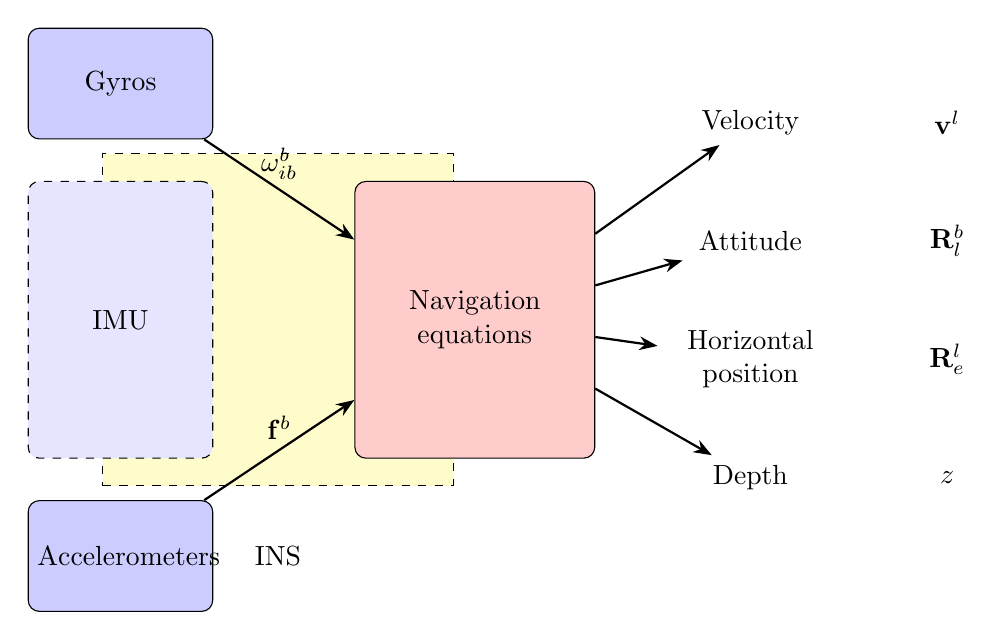
\begin{tikzpicture}[
    node distance=1.5cm,
    block/.style={rectangle, draw, fill=blue!20, text width=6em, text centered, rounded corners, minimum height=4em},
    block2/.style={rectangle, draw, fill=red!20, text width=8em, text centered, rounded corners, minimum height=10em},
    container/.style={rectangle, draw, dashed, fill=yellow!20, text width=12em, text centered, minimum height=12em},
    output/.style={rectangle, draw=none, text width=6em, text centered, minimum height=1em},
    arrow/.style={thick, ->, >=Stealth}
]

% INS container
\node[container] (INS) at (0,0) {};

% IMU container
\node[block, dashed, fill=blue!10, minimum height=10em, text width=6em] (IMU) at (-2,0) {IMU};

% Gyros
\node[block, above of=IMU, yshift=1.5cm] (Gyros) {Gyros};

% Accelerometers
\node[block, below of=IMU, yshift=-1.5cm] (Accel) {Accelerometers};

% Navigation equations
\node[block2, right of=IMU, xshift=3cm] (NavEq) {Navigation equations};

% Outputs
\node[output, right of=NavEq, xshift=2cm, yshift=2.5cm] (Vel) {Velocity};
\node[output, right of=NavEq, xshift=2cm, yshift=1cm] (Att) {Attitude};
\node[output, right of=NavEq, xshift=2cm, yshift=-0.5cm] (Pos) {Horizontal position};
\node[output, right of=NavEq, xshift=2cm, yshift=-2cm] (Depth) {Depth};

% Labels for outputs
\node[right of=Vel, xshift=1cm] (VelLabel) {$\mathbf{v}^l$};
\node[right of=Att, xshift=1cm] (AttLabel) {$\mathbf{R}_l^b$};
\node[right of=Pos, xshift=1cm] (PosLabel) {$\mathbf{R}_e^l$};
\node[right of=Depth, xshift=1cm] (DepthLabel) {$z$};

% Arrows from IMU to Navigation equations
\draw[arrow] (Gyros) -- node[above] {$\boldsymbol{\omega}_{ib}^b$} (NavEq);
\draw[arrow] (Accel) -- node[above] {$\mathbf{f}^b$} (NavEq);

% Arrows from Navigation equations to outputs
\draw[arrow] (NavEq) -- (Vel);
\draw[arrow] (NavEq) -- (Att);
\draw[arrow] (NavEq) -- (Pos);
\draw[arrow] (NavEq) -- (Depth);

% Labels for INS
\node[below of=INS, yshift=-1.5cm] {INS};

\end{tikzpicture}
\end{document}